\documentclass[1pt]{article}
\usepackage[utf8]{inputenc}
\usepackage{graphicx}
\usepackage{wrapfig}
\usepackage[left=.5in, right=.5in, top=.5in, bottom=.5in]{geometry}
\usepackage{subfig}
\usepackage{enumitem}
\usepackage{mathtools}
\usepackage{amssymb}
\usepackage{amsmath}
\usepackage{graphicx}
\usepackage{subcaption}
\usepackage{setspace}
\usepackage{float}
\usepackage[english]{babel}  % force American English hyphenation patterns
\usepackage{lmodern}


\renewcommand{\baselinestretch}{1} 
\newcommand{\norm}[1]{\left\lVert#1\right\rVert}
\DeclarePairedDelimiterX\set[1]\lbrace\rbrace{\def\given{\;\delimsize\vert\;}#1}

\graphicspath{ {pset2/images/} }

\title{6.867}
\author{Pset 2}
\date{}

\begin{document}
\maketitle

\section{   }

Here we consider linear regression given a set of  $N$ points $(X, y)$ (with $X_{ij} = x^{(i)}_j$, $y_i = y^{(i)}$, $X \in \mathbb{R}^{N \times d}, y \in \mathbb{R}^{N \times 1}$). We consider the ordinary least squares error function \\
$E^{OLS} = \sum_{i=1}^{N} (y^{(i)} - (w^Tx^{(i)} + w_0))^2 = \norm{y - Xw - (1)w_0}^2$\\
(where $(1)$ is the column vector of ones of length $N$) with its closed form solution\\
$\hat{w}^{OLS} = (X^TX)^{-1}X^Ty$ \\
$\hat{w_0}^{OLS} = \Bar{y} - \Bar{x}^Tw$ \\
as well as the ridge regression error function\\
$E^{Ridge} = E^{OLS} + \lambda \norm{w}^2$\\
and its closed form solution 
$\hat{w}^{Ridge} = (X^TX + \lambda I)^{-1}X^Ty$.
\begin{enumerate}[label=(\alph*)]
\item I now show that the same $\hat{w}^{Ridge}$ can be derived from the centered data. First, define the centered data to be \\
$X' = X - (1)\Bar{x}^T$\\
$y' = y - (1)\Bar{y}$\\
where
$\Bar{x} = \frac{1}{N}X^T(1)$ (the average $x^{(i)}$ vector) \\
$\Bar{y} = \frac{1}{N}y^T(1)$ (the average $y^{(i)}$ values) \\
And we know we are trying to minimize $E^{OLS}$, so if we substitute in $X'$ and $y'$ then we get \\
$\hat{w'}^{OLS} = (X'^TX')^{-1}X'^Ty'$. \\
But if we evaluate the error directly we see\\
$E^{OLS} =  \norm{y' - X'w - (1)w_0}^2$\\
$E^{OLS} =  \norm{y - (1)\Bar{y} - (X - (1)\Bar{x})^Tw - (1)w_0}^2$\\
$E^{OLS} =  \norm{(y - Xw) - (1)(\Bar{y} - \Bar{x}^Tw + w_0)}^2$\\
$E^{OLS} =  \norm{(y - Xw) - 2(1)w_0}^2$  since $w_0 = \Bar{y} - \Bar{x}^Tw$\\
$E^{OLS} =  \norm{(y - Xw)}^2$  since $w_0 = 0$\\
Thus the error term does not change and our optimal $w$ must also stay the same, ie \\
$\hat{w'}^{OLS} = (X'^TX')^{-1}X'^Ty' = (X^TX)^{-1}X^Ty = \hat{w}^{OLS}$. \\
We've seen that centering the data when $w_0 = 0$ does not change $\hat{w}^{OLS}$, which will allow me to now demonstrate an alternative interpretation of $\hat{w}^{Ridge}$. Define the augmented data set \\
$C = \begin{pmatrix}X'\\ \sqrt{\lambda} I_{d \times d} \end{pmatrix}$,
$Z = \begin{pmatrix}y'\\ (0)  \end{pmatrix}$ ($(0)$ being the length $d$ vector of zeros)\\
and see how we can substitute $C$ for $X$ and $Z$ for $y$, in essence adding artificial data which has response value zero, to shrink the components of $w$ and achieve the same results as ridge regression. Plugging these augmented matrices into the OLS error function yields  \\
$E^{OLS} =  \norm{Z - Cw - (1)w_0}^2$\\
$E^{OLS} =  \norm{\begin{pmatrix}y'\\ (0)  \end{pmatrix} - \begin{pmatrix}X'\\ \sqrt{\lambda} I_{d \times d} \end{pmatrix}w}^2$\\
$E^{OLS} =  \norm{y' - X'w}^2 +  \lambda \norm{w}^2$\\
$E^{OLS} =  \norm{y - Xw}^2 +  \lambda \norm{w}^2 = E^{Ridge}$\\
And so if the error function becomes the same as the error function for the ridge regression problem with pre-augmented $X$ and $y$, the solution must also be the same, thus, with $C$ and $Z$, \\
$\hat{w}^{Ridge} = (X^TX + \lambda I)^{-1}X^Ty$. 

\item Next we will see that the same ridge regression closed form solution for $w$ can be derived by instead considering this problem from a Bayesian perspective and choosing the $w$ which is most likely (under certain assumptions about the distribution of the data and possible $w$). We attempt to maximize \\
$P(w|D) \propto P(D|w) P(w)$\\
where\\
$D = {(x^{(i)}, y^{(i)})}$\\
$w \sim \mathcal{N}(0,\tau I)$\\
$y \sim \mathcal{N}(Xw,\sigma^2 I)$\\
$X_{ij} = x^{(i)}_j$\\
So now we can see that, given $X$, \\
$P(w|D) \propto e^{-\frac{1}{2 \sigma^2} \norm{y - Xw}^2 -\frac{1}{2 \tau} \norm{w}^2}$ \\
and to find the most likely $w$ (ie to maximize $P(w|D)$), maximize the value in the exponent, or minimize its negative, thus minimize \\
$\frac{1}{2 \sigma^2} \norm{y - Xw}^2 + \frac{1}{2 \tau} \norm{w}^2$ \\
which is the same as minimizing this value times a constant $ 2 \sigma^2$, thus we minimize \\
$\norm{y - Xw}^2 + \frac{\sigma^2}{\tau} \norm{w}^2$ \\
But this is the same form as the $E^{Ridge}$ we were trying to minimize earlier if we let $\frac{\sigma^2}{\tau} = \lambda$, thus the solution must be the same and \\
$\hat{w}^{Ridge} = (X^TX + \frac{\sigma^2}{\tau} I)^{-1}X^Ty = (X^TX + \lambda I)^{-1}X^Ty$. 

\end{enumerate}
\section{   }
In this question, we will show that neural networks with a $d$ dimensional input, one hidden layer, a one-dimensional output, and sigmoidal activation can approximate any continuous function $f : \mathbb{R}^d \rightarrow \mathbb{R}$ on the interval $[0, 1]^d$.
This proof relies on four steps. we'll prove two of these and then the rest will be given.
\begin{enumerate}[label=\arabic*.]
\item Let’s first suppose that we are given two functions $\rho : R \rightarrow R $ and $ \phi : R \rightarrow R$. We want to show that, if it possible to approximate $\phi$ using $span(H_\rho)$ in one dimension, then it is also possible to approximate $g \in H_\phi$ using $span(H_\rho)$ in $d$ dimensions. \\
More precisely, suppose that for any interval $[r, s]$ and any $tau > 0$, we can always find some $h \in  span(H_\rho)$ where
$sup \set{|h(x) - \phi(x)| : x \in [r, s]} \leq \tau$\\  
Note that here $h : R \rightarrow R$.\\
I now show that , for any $\epsilon  > 0 $ and any $g \in H_\phi$ with $g : \mathbb{R}^d \rightarrow \mathbb{R}$, we can choose some function $f \in span(H_\rho)$ where\\
$sup \set{|f(x) - g(x)| : x \in [0, 1]^d} \leq \epsilon$	\\
First, define $\theta, x' \in \mathbb{R}^d, b \in \mathbb{R}$ but restrict them so that $x' \in [0, 1]^d$ and $x = \theta^Tx'+b \in [r, s]$\\
Now substitute to get \\
$sup \set{|h(x) - \phi(x)| : x \in [r, s]} \leq \tau$\\ 
$sup \set{|\sum_i \alpha_i \rho(w_i x + b_i) - \phi(x)|} \leq \tau$\\
$sup \set{|\sum_i \alpha_i \rho(w_i (\theta^T x' + b) + b_i) - \phi(\theta^T x' + b)|} \leq \tau$\\ 
$sup \set{|\sum_i \alpha_i \rho(w_i \theta^T x' + (w_i b + b_i)) - \phi(\theta^T x' + b)|} \leq \tau$\\ 
let $w_i' = w_i \theta^T$  and  $b_i' = w_i b + b_i$\\
$sup \set{|\sum_i \alpha_i \rho(w_i'^T x' + b_i') - \phi(\theta^T x' + b)|: x' \in [0, 1]^d} \leq \tau$\\ 
$sup \set{|f(x') - g(x')|: x' \in [0, 1]^d} \leq \epsilon$\\ 
for $f \in span(H_\rho)$, $g \in H_\phi$, $\epsilon = \tau$. Thus step 1 is proved. 
\item Next, I prove that exp is Lipschitz continuous on any bounded
interval, so I'll show that there exists some real number $K \geq 0$ such that for any two real numbers $x_1$, $x_2$ in some given interval $[r, s]$, we have:\\
$|e^{x_2} - e^{x_1} | \leq K|x_2 - x_1|$\\
First, without loss of generality I shall assume that $x_2 > x_1$. Next, solve for $K$ and see that we need \\
$|e^{x_2} - e^{x_1} | / |x_2 - x_1| \leq K$\\
We know such a $K$ exists because $e^x$ and $|x_2 - x_1|$ are continuous for $x_2 \neq x_1$ (as assumed, for if $x_2 = x_1$ then the inequality is trivial), thus the MVT (Mean Value Theorem) applies for the interval $[x_1, x_2]$. Lets say the mean occurs at $x = x*$, then we can let $K = e^{x*}$ and the inequality must hold because the two sides become equal by definition of the mean over the interval.
\item The next two steps of the proof are not shown but they use steps one and two to show that one hidden layer neural networks with sigmoidal activation can approximate any continuous function on inputs in $[0, 1]^d$.
\end{enumerate}

\section{   }
For this section, we are analyzing the power of linear regression on a set of data $(x, y)$ where $x_i, y_i \in \mathbb{R}^M$, $0 \leq x \leq 1$, and $i \in \set{1, 2, ..., N}$ for $N = 11$. Points are sampled according
to the function \\
$y_i = cos(\pi x_i) + cos(2 \pi x_i) + \eta$\\
 for $\eta \sim \mathcal{N}(0,\sigma^{2})$ for small $\sigma$.\\
We analyze the effects of deriving solutions from closed form calculations as well as from gradient descent for the predictor $h(x) = w^T\phi(x)$ where $\phi, w \in \mathbb{R}^M$ and $ M \in \set{0, 1, ..., N}$ and the loss $L$ is calculated as \\
$L = \sum_{i=1}^N (h(x_i) - y_i)^2$

\begin{enumerate}[label=\alph*.)]
\item First we solve for $w$ with the closed from solution  \\
$w = (\Phi^T\Phi)^{-1} \Phi^T y$\\
for $\Phi(x) = (\phi(x_1), \phi(x_2), ..., \phi(x_N))^T$\\
and $\phi(x_i) = (1, x_i, x_i^2, ..., x_i^M)^T$\\
We see the effects of varying $M$ in Figure \ref{fig:3_1_a}. Though the underlying distribution is drawn from cosines, the small range allows these polynomial basis vectors to make good approximations for the underlying distribution under the small interval $[0, 1]$ for sufficiently large $M$.\\



% We see this reflected in the graph of the loss $L$ as a function of $M$; for small values of $M$ the loss is large but as $M$ increases it drops sharply. This continues until $M=2$, at which point the loss cannot go much lower and tapers off to $0$ as $M \to N$. This makes sense since we can see that, for the given sample interval, the underlying distribution goes through about half of a period and should therefore exhibit a nearly quadratic shape. Letting $M=2$ allows us to make a quadratic approximator, thus our approximator is under powered until this happens. We also can see that as we further increase $M$, we make very small improvements in reducing $L$. This is because, for the given model class (polynomials) and distribution range ($[0, 1]$), approximators of order greater than $M=2$ are too powerful so they find patterns in the data which don't exist. Thus the approximator over fits the points, marginally reducing $L$ but seriously increasing the complexity of the approximator and thus reducing generalizability.
\item Next, we observe the performance of gradient descent, batch gradient descent, and stochastic gradient descent using the SSE loss defined above. We compare the results to those obtained with the closed form solution above and also observe the effects of varying parameters in our gradient descent such as step size $\alpha$, convergence threshold $\delta$, and $w$ initialization $\w_{t=0}$. In Figure 2 we see gradient descent where each step's gradient was calculated using every point. Clearly the power of the model is retained - the curves for small $M$ were very similar to those derived using the closed form solution above. We also see that for $M=8$ the curve retains its simplicity - the complexity is more similar to that exhibited in Figure 1's third order polynomial than tenth order polynomial. This is because gradient descent has an inherent form of regularization within it; because there are increasingly many minima in the $M$ dimensional space of $E(w)$ as $M$ increases, it becomes increasingly likely that the $w$ vector will settle on some local, less extreme, point rather than the extremely deep, over-fitted point which optimally minimizes $E(w)$.\\
In Figure 4 we see we see we have reached the limit of batch gradient descent (here sgd is batch gradient descent but with batches of one) for the given hyperparameters. Even for $M=3$ and $M=8$ there simply were not enough points at each step to make a well informed step. As a result, there is essentially too much regularization and the model never finds a sufficiently deep $w$ to yield a good regression.\\

Next I analyze the effect of varying other model hyperparameters through the scope of loss rather than model geometry. \\
In the first plot of Figure 7 we see Loss plotted as a function of the convergence threshold $\delta$. Since $\delta$ dictates how little $w$ can change by on a step before we stop iterating, we should expect smaller $\delta$s to yield more refined $w$, and this is what we see. Further, we see that for higher order functions, a smaller $\delta$ seems to yield a smaller loss than for lower order functions. I would attribute this to the fact that the loss simply has a lower bound for higher order models since their higher capacity for complexity allow them to conform more tightly to the data. \\
The next plot shows loss as a function of step size $\alpha$. Since step size determines the granularity of the steps we are able to make in searching for wells in $E(w)$, we should expect to be able to find more elusive wells with a smaller step size (as a larger step size would just cause us to overshoot the well and jump into some unrelated section of the surface). Indeed, we see that for sm
The final plot shows loss as a function of the standard deviation with which the $w$ vector's values are initialized (pulled from a normal distribution). The plot would suggest that for very small standard deviations the algorithm is still able to find a good $w$. We see that as the initialization standard deviation gets larger, performance suffers, indicating that the values it is initialized with are so large in magnitude that they are never close enough to the true values to approach a good solution. \\

\item Finally, lets now assume we know the distribution's basis functions take the form $ cos(i \pi x)$. We first set $\phi(x_i) = (cos(\pi x_i), cos(2 \pi x_i),  ... , cos(M \pi x_i))^T$ and see whether our model can extract the coefficients in $w$ which match those from which the distribution was generated ($w = (1, 1, 0, 0, ...., 0)^T$ using the closed form solution for $w$. We then do the same thing using the same $\phi(x_i)$ except with an additional element $1$ at the beginning to see how this affects our result. \\


\centerline{Weight Vector Coefficients (no Constant Term)}
\begin{align*}
* & : & 1 & & 1 & &  \\
1 & : & 0.779 & &   & & \\
2 & : & 0.779 & & 1.174 & &  \\
3 & : & 0.763 & & 1.174 & & 0.094 \\
4 & : & 0.763 & & 1.141 & & 0.094 & & 0.197 \\
5 & : & 0.77 & & 1.141 & & 0.101 & & 0.197 & & -0.049 \\
6 & : & 0.77 & & 1.089 & & 0.101 & & 0.145 & & -0.049 & & 0.363 \\
7 & : & 0.769 & & 1.089 & & 0.099 & & 0.145 & & -0.051 & & 0.363 & & 0.012 \\
8 & : & 0.769 & & 1.087 & & 0.099 & & 0.143 & & -0.051 & & 0.362 & & 0.012 & & 0.015
\end{align*}
We see that in this basis we require a similar number of dimensions for $\phi$ to be able to approximate the true distribution function When we directly inspect the optimal weight vectors we see that the coefficients for $ cos(\pi x)$ and  $ cos(2 \pi x)$ are nearly $1$ while the others are closer to zero, as we should hope. Interestingly, the coefficient for the sixth term is unexpectedly large for $M \geq 6$, though we know the sample distribution so it must have randomly generated noise with an approximate frequency of $6$. 

% \begin{figure}[H]
%   \begin{subfigure}
%     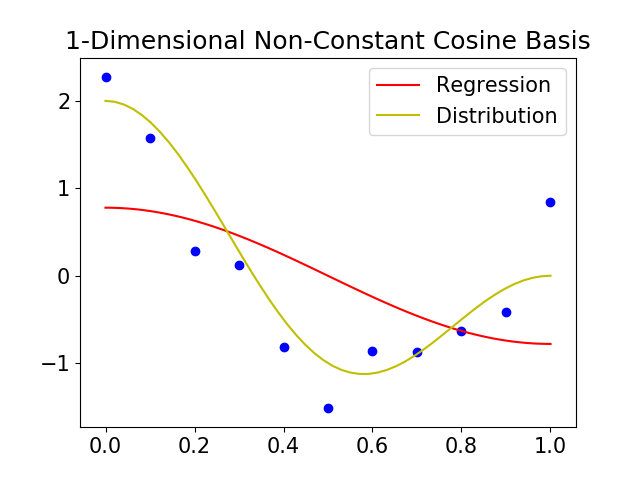
\includegraphics[width=.3\linewidth]{const_cosine_basis_1.png}
%     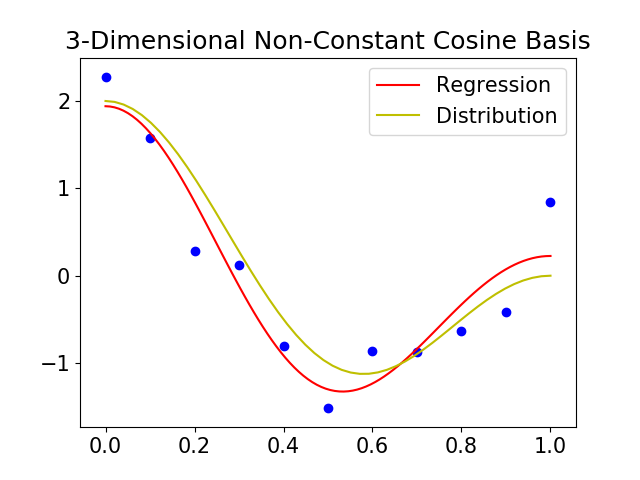
\includegraphics[width=.3\linewidth]{const_cosine_basis_3.png}
%     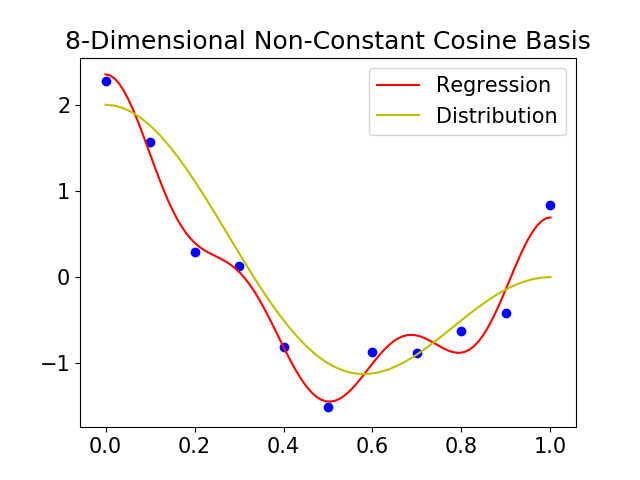
\includegraphics[width=.3\linewidth]{const_cosine_basis_8.png}
%     \caption{Cosine Basis with Constant Term}
%   \end{subfigure}
%   \label{fig:3_3_a}
% \end{figure}\\

% \centerline{Weight Vector Coefficients (with Constant Term)}
% \begin{align*} \\
% * & : & 0 & & 1 & & 1 \\
% 0 & : & -0.001 \\
% 1 & : & -0.001 & & 0.779 \\
% 2 & : & -0.109 & & 0.779 & & 1.192 \\
% 3 & : & -0.109 & & 0.763 & & 1.192 & & 0.094 \\
% 4 & : & -0.126 & & 0.763 & & 1.159 & & 0.094 & & 0.215 \\
% 5 & : & -0.126 & & 0.77 & & 1.159 & & 0.101 & & 0.215 & & -0.049 \\
% 6 & : & -0.151 & & 0.77 & & 1.108 & & 0.101 & & 0.164 & & -0.049 & & 0.382 \\
% 7 & : & -0.151 & & 0.769 & & 1.108 & & 0.099 & & 0.164 & & -0.051 & & 0.382 & & 0.012 \\
% 8 & : & -0.153 & & 0.769 & & 1.104 & & 0.099 & & 0.16 & & -0.051 & & 0.379 & & 0.012 & & 0.032 \\
% \end{align*}\\

% Here we see the added constant term hardly changes the graphs. This is as we should expect since the underlying distribution the data was generated from did not have a constant term. Inspecting the $w$ values confirms this as the magnitudes of the constant term coefficient are all small while the other coefficients are similar to the ones from the previous tests without the constant term. \\


\end{enumerate}
\section{   }
In this section we are analyzing a series of CNNs used to categorize pictures of ten different articles of clothing.
\begin{enumerate}[label=\arabic*.]
\item \begin{enumerate}[label=(\alph*)]
\item For Alice, ten epochs of training yielded a training error $E_{Train}$ of $.90$ and testing error $E_{Test}$ of $.89$. \\
Her CNN was organized as like so:\\
$x \rightarrow_1 C_1 \rightarrow_2 C_2 \rightarrow_3 L_1 \rightarrow_4 L_2 \rightarrow_5 L_3 $\\
input $x$ was the 28x28 image\\
transition 1 was convolution with one input channel, ten output channels, stride of two, kernel size of five, and max pooling ReLU activation \\
$C_1$ was a 12x12x10 tensor\\
transition 2 was convolution with ten input channels, twenty output channels, stride of two, kernel size of five, and max pooling ReLU activation \\
$C_2$ was a 4x4x20 tensor\\
transition 3 was flattening to a 320x1 vector\\
$L_1$ was a 320x1 vector\\
transition 4 was a dense layer with input 320x1, output 50x1, and ReLU activation\\
$L_2$ was a 50x1 vector\\
transition 5 was a dense layer with input 50x1, output 10x1, and softmax activation\\
$L_3$ was a 10x1 vector trained by NLL (negative log likelihood)\\
Her final hyperparameter was the learning rate of the network, which was 0.00001. 
\item Her training error was far too low, her network never had a chance of making significant progress toward a strong solution. Over ten epochs, I achieved my minimum testing error of 0.13 by setting the learning rate to 0.1.
\item From experimenting with various values for the learning rate I found that, starting from her initial rate of 0.00001, increasing the learning rate decreased the error. Presumably this was because the model was able to move more quickly along the surface through gradient descent (and also able to escape too shallow of wells, freeing it from shallow local minima which would yield weak solutions). The learning rate can get too high, however, at which point the model changes too much between iterations and is never able to settle into a good solution. We can see from the first plot in Figure 8 that the optimal learning rates seem to be between .01 and .5. 
\end{enumerate}
\item Now we analyze Bob's CNN, which doesn't perform as well as Alice's. 
\begin{enumerate}
    \item For Bob, ten epochs of training yielded a training error $E_{Train}$ of $.45$ and testing error $E_{Test}$ of $.47$.\\
    His architecture is the same as Alice's except the final output was activated by ReLU (and rounded to an integer for the class prediction) and the network was trained on MSE (Mean Square Error) Loss.
    \item Bob was trying to solve this problem like a regression problem. We can see this is the case in line 33 where the final return of a pass through the net is \begin{verbatim} return F.relu(x) \end{verbatim} (rather than softmax) and in line 33 where he chooses NLL loss: \begin{verbatim} loss = F.nll_loss(output, target) \end{verbatim}
    showing that he is treating the classes as members of some continuous, one dimensional spectrum.
    \item Bob is solving the wrong problem because the pictures are members of discrete classes, not a continuous spectrum. To do regression on them is to imply structure which they do not exhibit. Rather, classes are all equally pairwise distinct, thus they should be assigned their own dimensions, as they are when using one hot vectors. The solution is therefore to use softmax with softmax and NLL as Alice did since this makes the correct assumptions about the underlying structure of the data. 
\end{enumerate}
\item Now we Chelsea's CNN along with her hypothesis that small training set sizes $N$ are sufficient to build good models. 
\begin{enumerate}
    \item I am doubtful because this seems like a very small amount of data to capture the intricacies of ten different classes and also because it is very possible to get flukes in training whereby a model misleadingly tests well on the test set even though it cannot truly generalize well. I would be less incredulous if I knew how much she tested the model. 
    \item Looking down at Figure 9, it is clear that, while the model frequently never finds a strong solution by the end of the twenty-five epochs, when it does find a decent solution that solution is likely to be better if $N$ is larger. Ignoring the times when the model couldn't find a solution, all of the plots indicate an asymptotic improvement in the target value (be it minimizing Loss or maximizing Accuracy). In fact, the asymptotes seem to be unreached in the plots, implying that the ideal $N$ is actually greater than $60000$ if training time is not an issue (if it is, then $N = 3000$ seems to be a good compromise between accuracy and parsimony in sampling). 
\end{enumerate}
\item Now we see the performance of Daniel's network on his real world data.
\begin{enumerate}
    \item After ten epochs, training and test accuracy were .91 and .90 while the model only achieved an accuracy of .50. 
    \item To improve the accuracy we could artificailly rotate the testing set so that it can better account for rotation in Daniels real world data. 

\end{enumerate}
\end{enumerate}

\begin{figure}[h!]
\centering
  \begin{subfigure}
    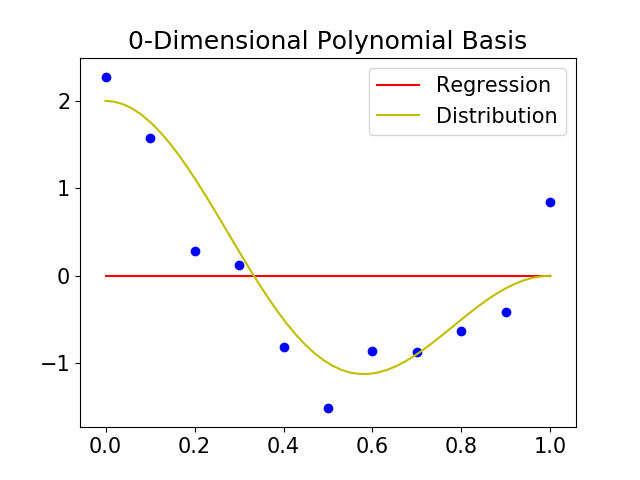
\includegraphics[width=.24\linewidth]{poly_basis_0.png}
    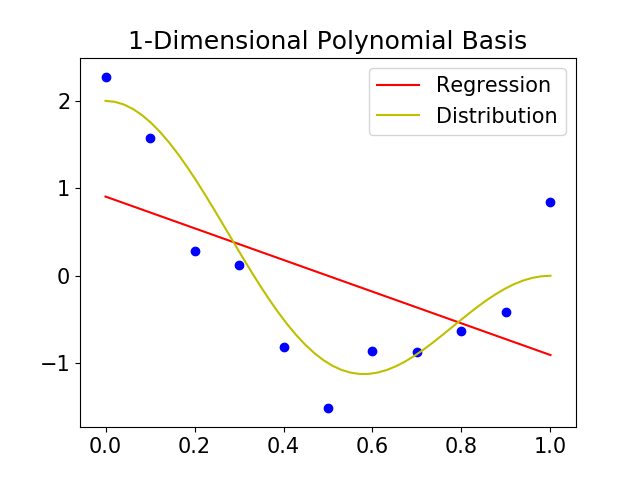
\includegraphics[width=.24\linewidth]{poly_basis_1.png}
    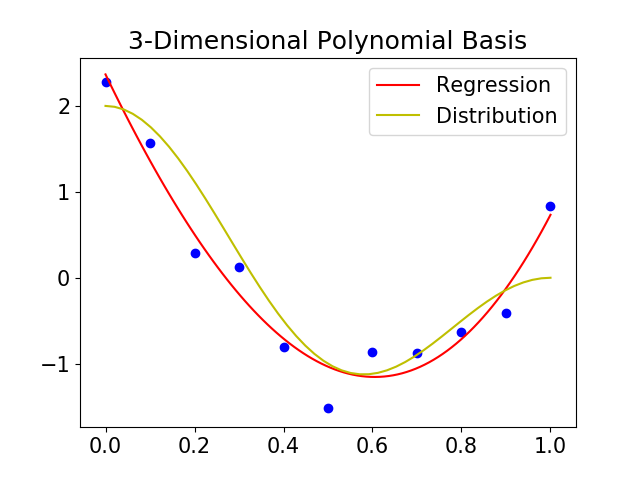
\includegraphics[width=.24\linewidth]{poly_basis_3.png}
    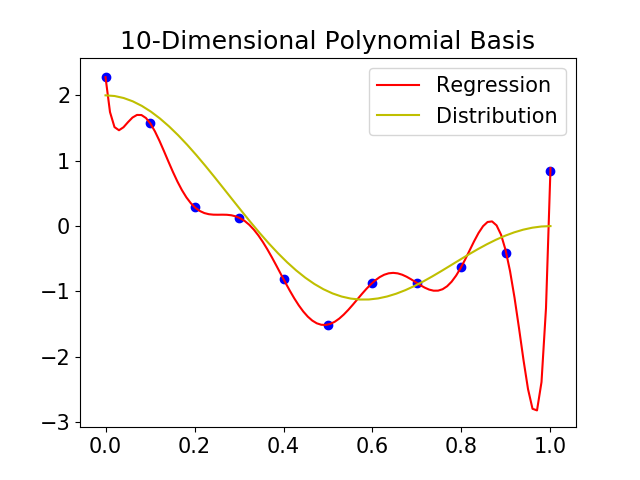
\includegraphics[width=.24\linewidth]{poly_basis_10.png}
  \end{subfigure}
  \caption{Polynomial Regression}
  \label{fig:3_1_a}
\end{figure}

\begin{figure}[H]
\centering
  \begin{subfigure}
    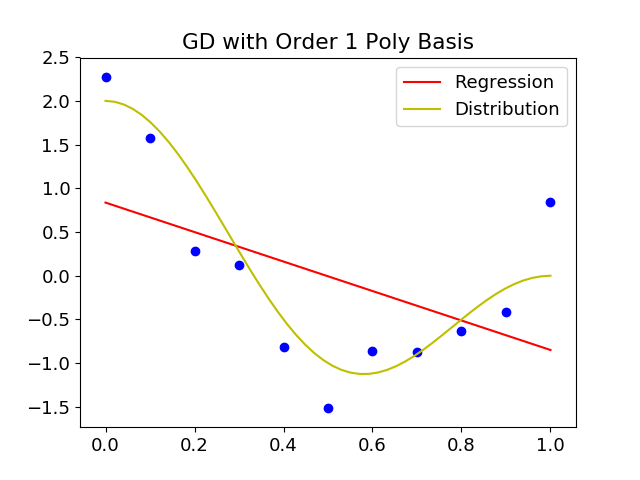
\includegraphics[width=.25\linewidth]{gd1.png}
    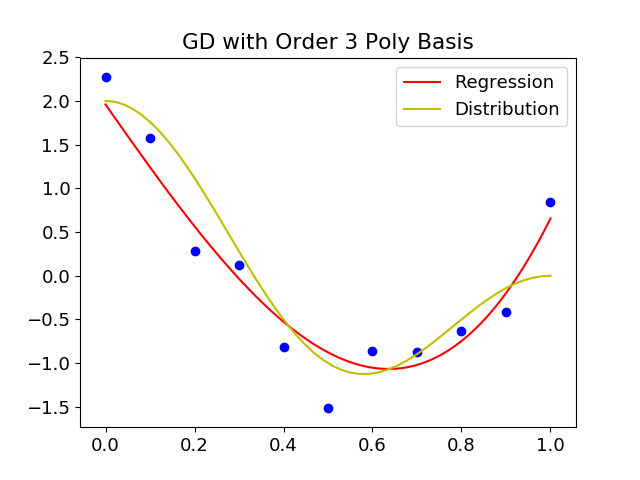
\includegraphics[width=.25\linewidth]{gd3.png}
    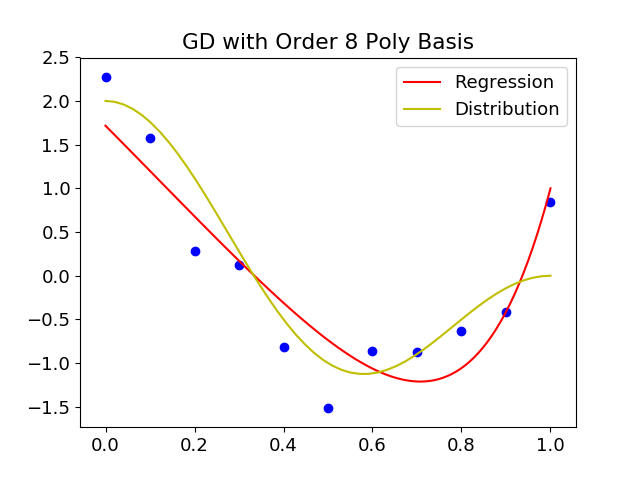
\includegraphics[width=.25\linewidth]{gd8.png}
    \caption{Gradient Descent}
  \end{subfigure}
  \begin{subfigure}
    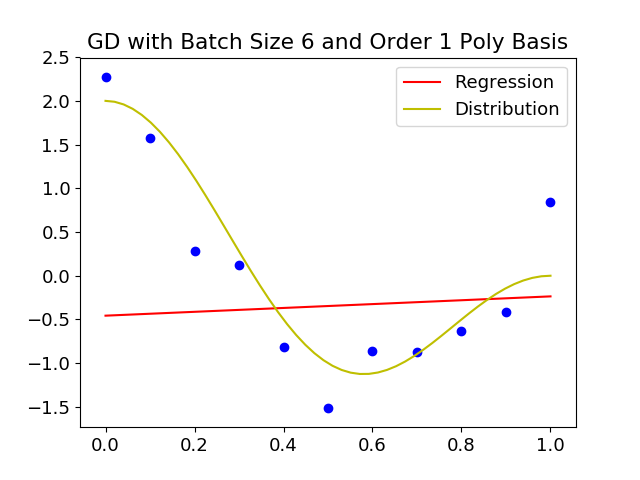
\includegraphics[width=.25\linewidth]{gd61.png}
    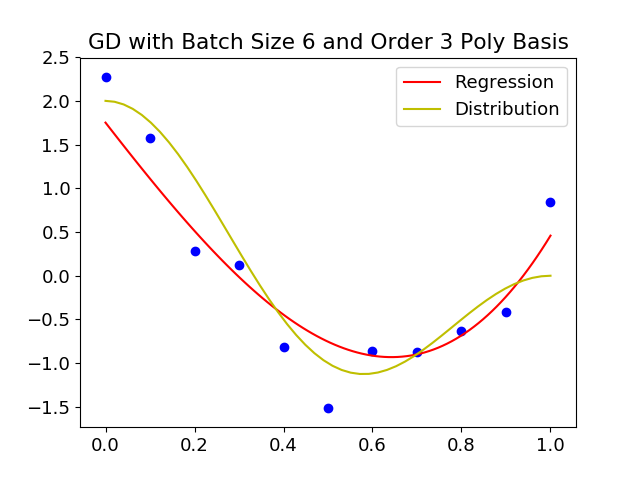
\includegraphics[width=.25\linewidth]{gd63.png}
    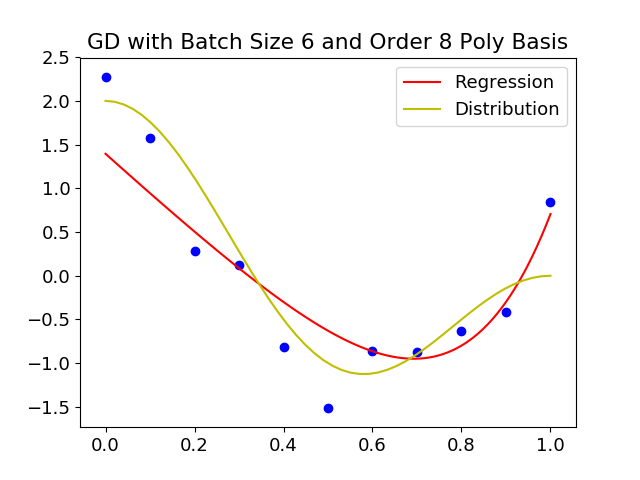
\includegraphics[width=.25\linewidth]{gd68.png}
    \caption{Batch Gradient Descent (Batch Size = 6)}
  \end{subfigure}
  \begin{subfigure}
    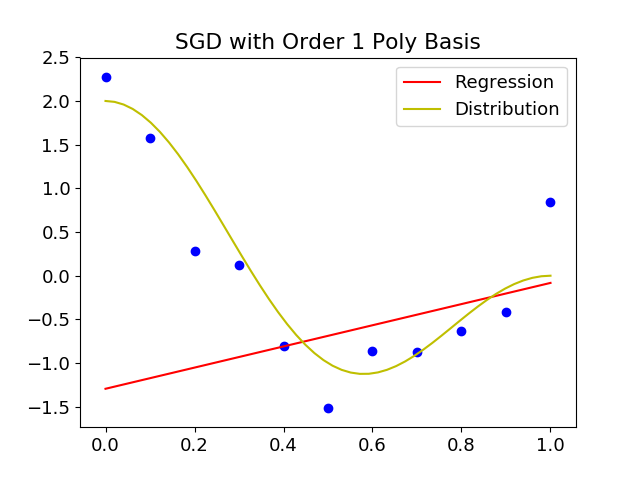
\includegraphics[width=.25\linewidth]{sgd1.png}
    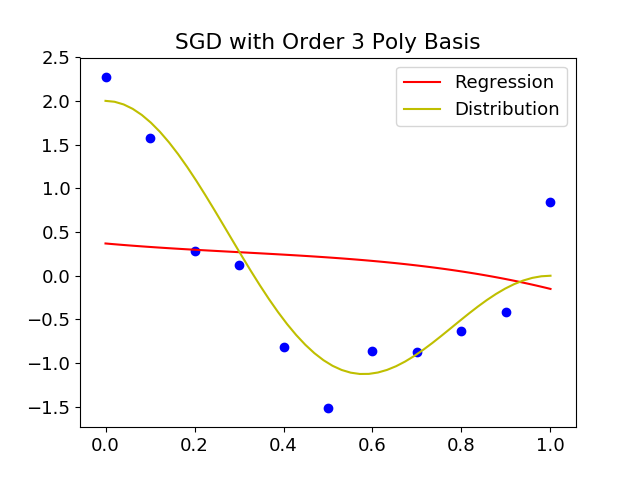
\includegraphics[width=.25\linewidth]{sgd3.png}
    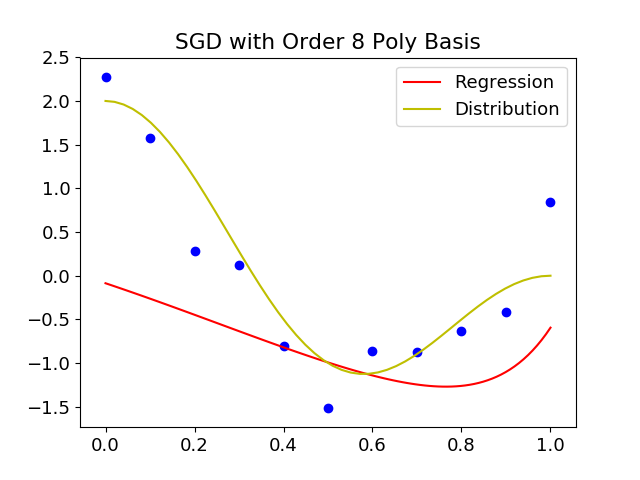
\includegraphics[width=.25\linewidth]{sgd8.png}
      \caption{Stochastic Gradient Descent}
  \end{subfigure}
  \caption{Gradient Descent with Various Batch Sizes and Fixed $\alpha = .001$, $w_{t=0} \sim \mathcal{N}(0,1)$, $\delta = .0001$}
  \label{fig:3_2_a}
\end{figure}\\

\begin{figure}[H]
\centering
  \begin{subfigure}
    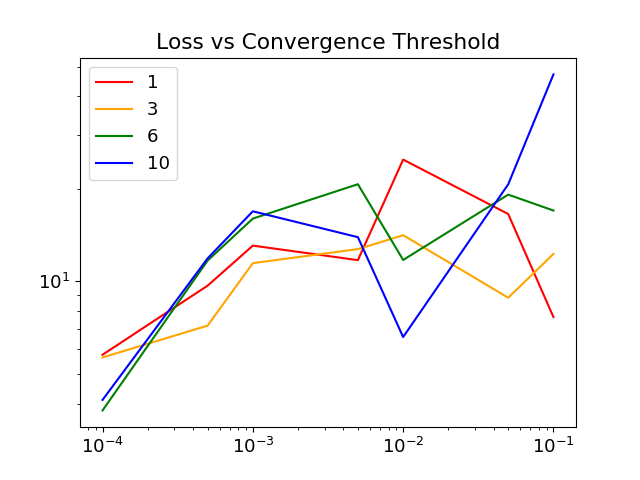
\includegraphics[width=.3\linewidth]{delta.png}
    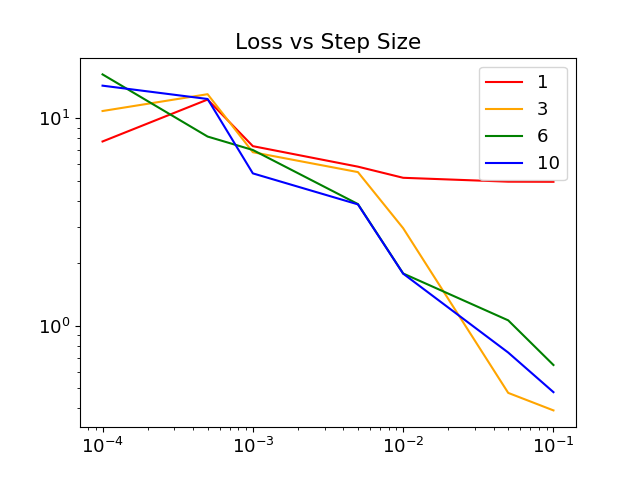
\includegraphics[width=.3\linewidth]{alphas.png}
    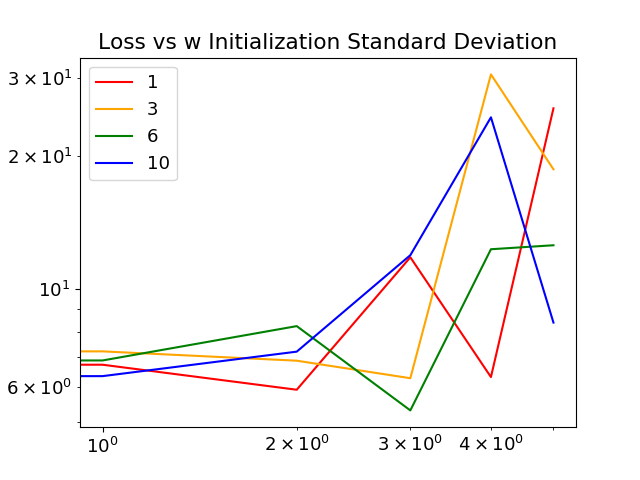
\includegraphics[width=.3\linewidth]{w_init.png}
  \end{subfigure}
  \caption{Gradient Descent with Varied Hyperparameters}
  \label{fig:3_2_b}
\end{figure}

\begin{figure}[H]
\centering
  \begin{subfigure}
    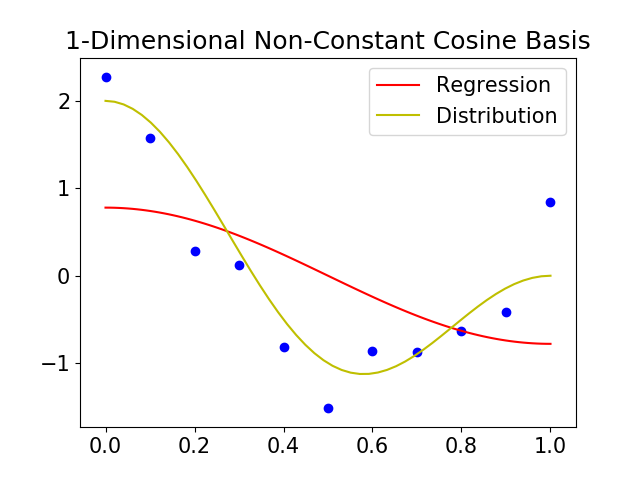
\includegraphics[width=.3\linewidth]{cosine_basis_1.png}
    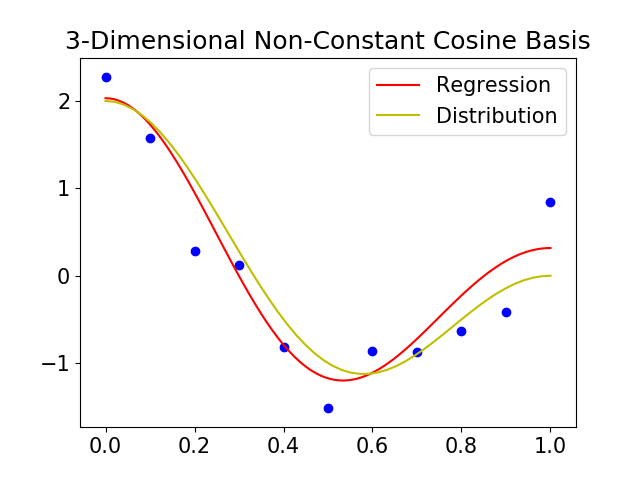
\includegraphics[width=.3\linewidth]{cosine_basis_3.png}
    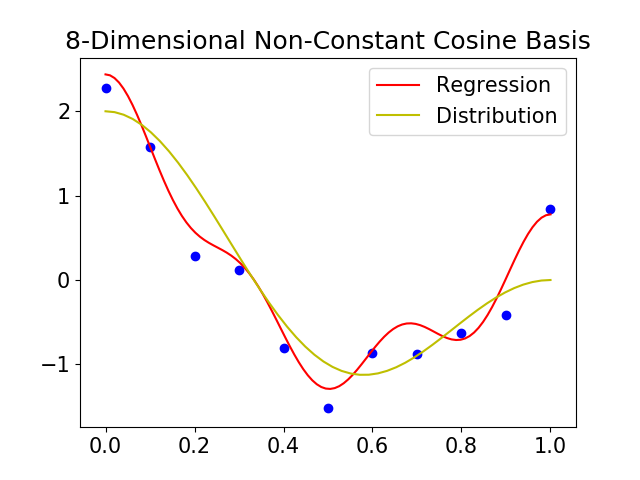
\includegraphics[width=.3\linewidth]{cosine_basis_8.png}
    \caption{Cosine Basis with no Constant Term}
  \end{subfigure}
  \label{fig:3_3_a}
\end{figure}

\begin{figure}[H]
\centering
  \begin{subfigure}
    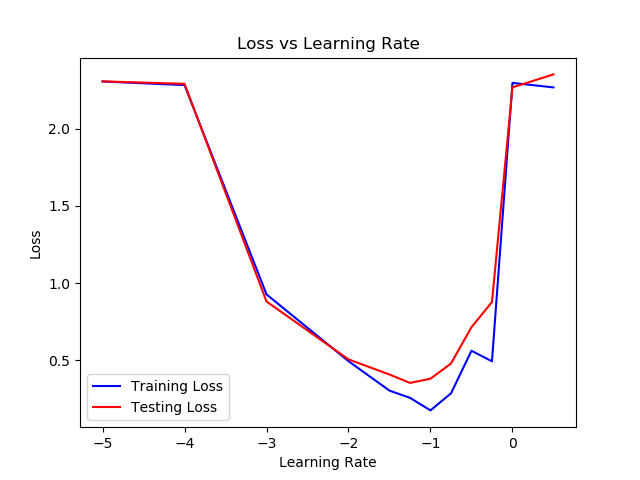
\includegraphics[width=.3\linewidth]{4_1_a.png}
    \caption{Loss vs Learning Rate in Alice's NN}
\end{subfigure}
\begin{subfigure}
    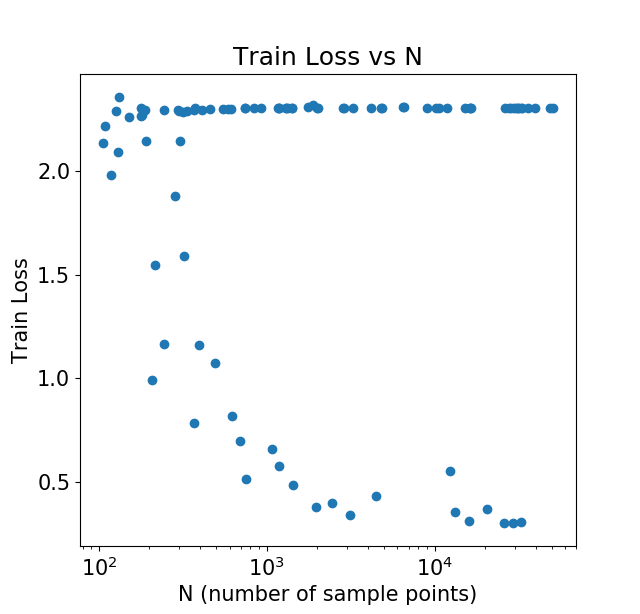
\includegraphics[width=.24\linewidth]{3_train_loss_N.png}
     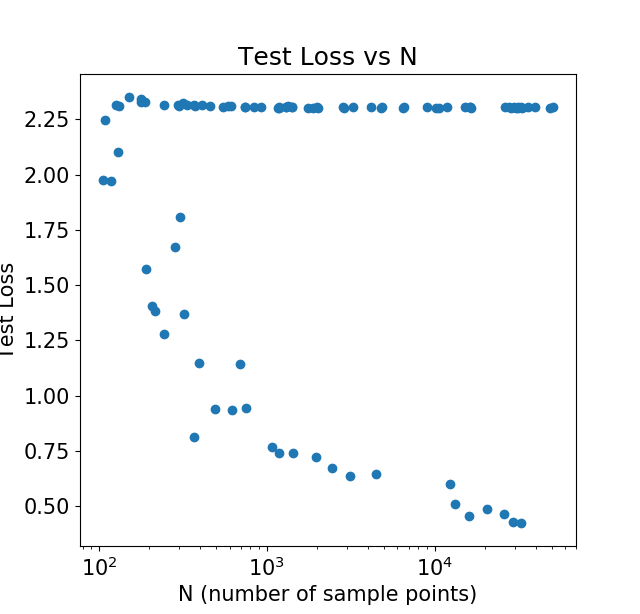
\includegraphics[width=.24\linewidth]{3_test_loss_N.png}
    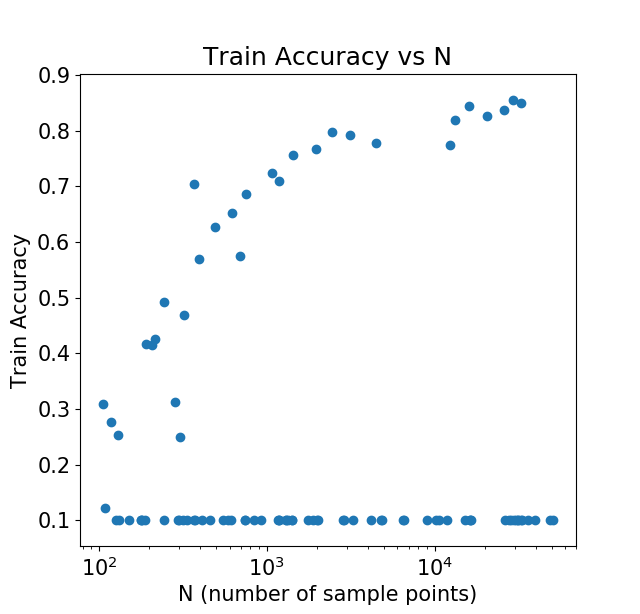
\includegraphics[width=.24\linewidth]{3_train_acc_N.png}
    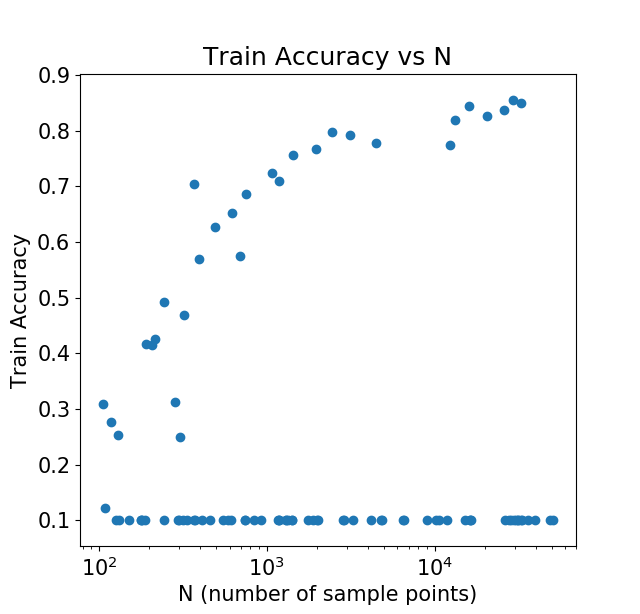
\includegraphics[width=.24\linewidth]{3_train_acc_N.png}
    \caption{Loss and Accuracy as a Function of N}
  \end{subfigure}
\end{figure}

\end{document}